% \documentclass[12pt, border = 8pt, varwidth, convert]{standalone}
\documentclass[margin=3pt,
   varwidth, 
  convert,
  convert={
    outext=.png,
    command=\unexpanded{
      pdftocairo -r 300 -png \infile % 将生成的pdf文件转换为png图像
    }
  }
  ]{standalone}

\usepackage{tkz-fct}
\usepackage{tkz-euclide}% 绘制线段命令(此处仅标注尺寸)

\begin{document} %在document环境中撰写文档
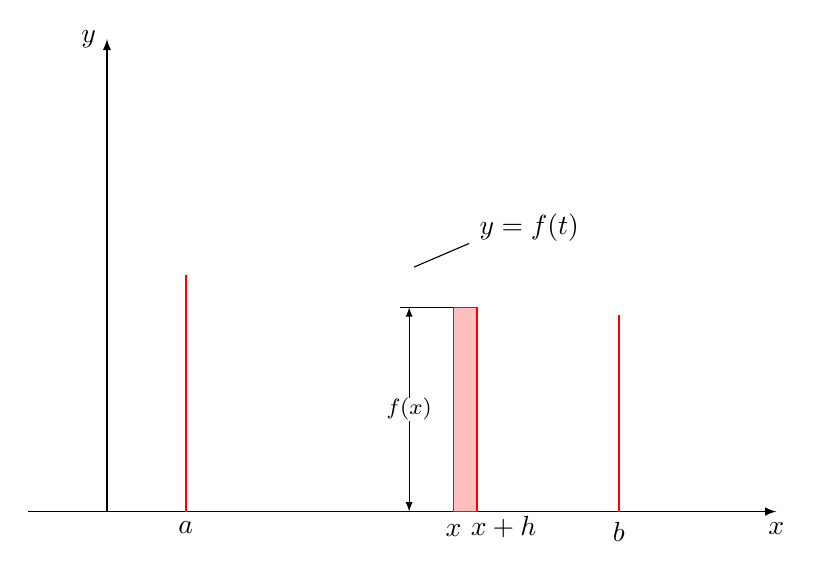
\begin{tikzpicture}
  % 定义坐标区域
  \tkzInit[xmin=-1, xmax=8, ymin=0, ymax=5.5]
  % 绘制坐标轴
  \tkzDrawXY[noticks]
  % 绘制曲线
  \tkzFct[thick,color=cyan, domain=1:6.5]{sin(pi/3*(x-1))+3}
  % 定义坐标点
  \tkzDefPointByFct(1) \tkzGetPoint{a}
  \tkzDefPointByFct(6.5) \tkzGetPoint{b}
  \tkzDefPointByFct(4.4) \tkzGetPoint{c}
  \tkzDefPoint(4.4,0){d}
  \tkzDefPointByFct(3.9) \tkzGetPoint{e}
  % 绘制线段
  \draw[thick, red](1,0) -- (a);
  \draw[thick, red](6.5,0) -- (b);
  % 标记各个点
  \tkzLabelPoint[below](1,0){$a$}
  \tkzLabelPoint[below](6.5,0){$b$}
  \tkzLabelPoint[below,shift={(0.0pt, -1.1pt)}](4.4,0){$x$}
  \tkzLabelPoint[below right,shift={(-6.0pt, 2.0pt)}](4.7,0){$x+h$}
  % 绘制区域
  \tkzDrawSegment[dim={$f(x)$,16pt, transform shape}](d,c)
  \fill[draw=red, fill=red!50, fill opacity=0.5](c) rectangle (4.7, 0);
  % 绘制填充区域  
  \tkzDrawArea[opacity=0.3, color=cyan!50, domain =1:6.5]
  % 绘制函数名称
  \draw[black](e)--+(0.7, 0.3)node[anchor=south west, yshift=-3pt]{$y=f(t)$};
\end{tikzpicture}

\begin{tikzpicture}[scale=2]
  % 定义坐标区域
  \tkzInit[xmin=0, xmax=2,xstep=1, ymin=-4, ymax=8,ystep=4]  
  % 设置坐标轴刻度
  \tkzSetUpAxis[tickwd=0.5pt,ticka=2pt, tickb=0pt]
  % 绘制坐标轴
  \tkzAxeXY
  % 绘制曲线
  \tkzFct[name path global=A, thick,color=cyan, domain=0:2]{9*x**2-16*x+4}
  \tkzFct[domain=0:2]{0}
  % 定义路径
  \path[name path global= B](0,0)--(2,0);
  % % 求交点
  \path[black,name intersections={of=A and B,by={[label=below left:$c$]C, [label=below right:$c$]C'}}];
  \tkzDrawAreafg[between= a and b,color=cyan!50]
  \tkzDrawAreafg[between= b and a,color=orange!50]
  \tkzText[black](1.5, 8.5){$y = f(x) = 9x^2 - 16x + 4$}
\end{tikzpicture}
\end{document}

%%% Local Variables:
%%% mode: latex
%%% TeX-master: t
%%% End:
